\chapter{Construction of Wiener Measure}\label{chap4}

ONE\pageoriginale EXAMPLE WHERE the Kolmogorov construction yields a
probability measure concentrated on a ``nice'' class $\Omega$ is the
Brownian motion.

\begin{defi*}
A Brownian motion with starting point $x$ is an
$\mathbb{R}^{d}$-valued stochastic process $\{X(t):0\leq t<\infty\}$
where
\begin{itemize}
\item[(i)] $X(0)=x=$ constant;

\item[(ii)] the family of distribution is specified by
\begin{align*}
F_{t_{1}}\ldots
t_{k}(A) &=
\int\limits_{A}p(0,x,t_{1},x_{1})p(t_{1},x_{1},t_{2},x_{2})\ldots\\
&\quad 
p(t_{k-1},x_{k-1},t_{k},x_{k})dx_{1}\ldots dx_{k}
\end{align*}
for every Borel set $A$ in $\mathbb{R}^{d}\times\cdots\mathbb{R}^{d}$
($k$ times).
\end{itemize}
\end{defi*}

\noindent
{\bf N.B.}~ The stochastic process appearing in the definition above
is the one given by the Kolmogorov construction.

It may be useful to have the following picture of a Brownian
motion. The space $\Omega_{k}$ may be thought of as representing
particles performing Brownian movement; $\{X_{t}:0\leq t<\infty\}$
then represents the trajectories of these particles in the space
$\mathbb{R}^{d}$ as functions of time and $\mathscr{B}$ can be
considered as a representation of the observations made on these
particles.

\begin{exercise}\label{chap4-exer2}
\begin{enumerate}
\renewcommand{\theenumi}{\alph{enumi}}
\renewcommand{\labelenumi}{(\theenumi)}
\item Show that $F_{t_{1}\ldots t_{k}}$ defined above is a probability
  measure on $\mathbb{R}^{d}\times\cdots\times \mathbb{R}^{d}$ ($k$
  times).

\item $\{F_{t_{1}\ldots t_{k}}:0\leq t_{1}<t_{2}<\ldots t_{k}<\infty\}$
  satisfies the consistency condition. (Use Fubini's theorem).

\item $X_{t_{1}}-x$,\pageoriginale
  $X_{t_{2}}-X_{t_{1}},\ldots,X_{t_{k}}-X_{t_{k-1}}$ are independent random
  variables and if $t>s$, then $X_{t}-X_{s}$ is a random variable
  whose distribution density is given by
$$
p(t-s,y)=\frac{1}{[2\pi(t-s)]^{d/2}}\exp\left(-\frac{1}{2}(t-s)^{-1}|y|^{2}\right).
$$
(Hint: Try to show that $X_{t_{1}}-x$,
$X_{t_{2}}-X_{t_{1}},\ldots,X_{t_{k}}-X_{t_{k-1}}$ have a joint
distribution given by a product measure. For this let $\phi$ be any
bounded real measurable function on $\mathbb{R}^{d}\times\cdots\times
\mathbb{R}^{d}$ ($k$ times). Then
$$
{\displaystyle{\mathop{E(\phi(Z_{1},\ldots,Z_{k}))}_{X_{t_{1}}-x,X_{t_{2}}-X_{t_{1}},\ldots,X_{t_{k}}-X_{t_{k-1}}}}}={\displaystyle{\mathop{E}_{X_{t_{1}},\ldots,X_{t_{k}}}}}(\phi(Z_{1}-x,\ldots,Z_{k}-Z_{k-1}))
$$
where ${\displaystyle{\mathop{E(\phi)}_{X_{t_{1}}\ldots X_{t_{k}}}}}$ is the
expectation of $\phi$ with respect to the joint distribution of
$(X_{t_{1}}\ldots,X_{t_{k}})$. You may also require the change of
variable formula).
\end{enumerate}
\end{exercise}

\begin{problem*}
Given a Brownian motion with starting point $x$ our aim is to find a
probability $P_{x}$ on the space $\Omega=C([0,\infty);\mathbb{R}^{d})$
  of all continuous funcitons from $[0,\infty)\to \mathbb{R}^{d}$
    which induces the Brownian motion. We will thus have a {\em
      continuous realisation} to Brownian motion. To achieve this goal
    we will work with the collection $\{F_{t_{1},\ldots,t_{k}}:0\leq
    t_{1}<t_{2}<\ldots<t_{k}\}$ where $t_{i}\in D$, a countable dense
    subset of $[0,\infty)$.
\end{problem*}

\setcounter{step}{0}
\begin{step}%1
The\pageoriginale first step is to find a probability measure on a
``smaller'' space and lift it to $C([0,\infty);\mathbb{R}^{d})$. Let
$$
\Omega=C([0,\infty);\mathbb{R}^{d}),
$$
$D$ a countable dense subset of $[0,\infty)$; $\Omega(D)=\{F:D\to
    \mathbb{R}^{d}\}$ where $f$ is uniformly continuous on $[0,N]\cap
    D$ for $N=1,2,\ldots$. We equip $\Omega$ with the topology of
    uniform convergence on compact sets and $\Omega(D)$ with the
    topology of uniform convergence on sets of the form $D\cap K$
    where $K\subset [0,\infty)$ is compact; $\Omega$ and $\Omega(D)$
      are separable metric spaces isometric to each other.
\end{step}

\begin{exercise}\label{chap4-exer3}
Let
$$
p_{n}(f,g)=\sup\limits_{0\leq t\leq n}|f(t)-g(t)|\quad\text{for}\quad
f,g\in \Omega
$$
and 
$$
p_{n,D}(f,g)=\sup\limits_{\substack{0\leq t\leq n\\ t\in
    D}}|f(t)-g(t)|\quad\text{for}\quad f,g\in \Omega(D).
$$

Define
\begin{align*}
\rho(f,g) &=
\sum^{\infty}_{n=1}\frac{1}{2^{n}}\frac{p_{n}(f,g)}{1+p_{n}(f,g)},\ \forall
f,g\in \Omega,\\
\rho_{D}(f,g) &=
\sum^{\infty}_{n=1}\frac{1}{2^{n}}\frac{p_{n,D}(f,g)}{1+p_{n,D}(f,g)},\ \forall
f,g\in \Omega(D).
\end{align*}


Show that
\begin{enumerate}
\renewcommand{\theenumi}{\roman{enumi}}
\renewcommand{\labelenumi}{(\theenumi)}
\item $\{f_{n}\}\subset \Omega$ converges to $f$ if and only if
  $f_{n}\to f$ uniformly on compact subsets of $[0,\infty)$;

\item $\{f_{n}\}\subset \Omega(D)$ converges to $f$ if and only if
  $f_{n|D\cap K}\to f_{|D\cap K|}$ uniformly for every compact subset
  $K$ of $[0,\infty)$;

\item $\{(P_{1},\ldots,P_{d})\}$\pageoriginale where $P_{i}$ is a
  polynomial with rational coefficients is a countable dense subset of
  $\Omega$; 

\item $\{(P_{1D},\ldots,P_{dD})\}$ is a countable dense subset of
  $\Omega(D)$;

\item $\tau:\Omega\to \Omega(D)$ where $\tau(f)=f_{|D}$ is a
  $(\rho,\rho_{D})$-isometry of $\Omega$ onto $\Omega(D)$;

\item if $V(f,\epsilon,n)=\{g\in \Omega:p_{n}(f,g)<\epsilon\}$ for
  $f\in \Omega$, $\epsilon>0$ and
$$
V_{D}(f,\epsilon,n)=\{g\in\Omega(D):p_{n,D}(f,g)<\epsilon\}\quad\text{for}\quad
f\in \Omega(D), \epsilon>0,
$$
then
$$
\{V(f,\epsilon,n):f\in \Omega,\epsilon>0,n=1,2\ldots\}
$$
is a base for the topology of $\Omega$ and
$$
\{V_{D}(f,\epsilon,n):f\in \Omega(D),\epsilon>0,n=1,2,\ldots\}
$$
is a base for the topology of $\Omega(D)$.
\end{enumerate}
\end{exercise}

\begin{remark*}
By Exercise \ref{chap4-exer3}(v) any Borel probability measure on
$\Omega(D)$ can be lifted to a Borel probability measure on $\Omega$.
\end{remark*}

\noindent
{\bf 2nd Step.}~ Define the modulus of continuity
$\Delta^{T,\delta}_{D}(f)$ of a function $f$ on $D$ in the interval
$[0,T]$ by
$$
\Delta^{T,\delta}_{D}(f)=\sup \{|f(t)-f(s)|:|t-s|<\delta t,s\in D\cap
      [0,T]\}
$$

As $D$ is countable one has

\begin{exercise}\label{chap4-exer4}
\begin{enumerate}
\renewcommand{\theenumi}{\alph{enumi}}
\renewcommand{\labelenumi}{(\theenumi)}
\item Show that $f:\Delta^{N,\frac{1}{j}}_{D}(f)\leq \frac{1}{k}\}$ is
  measurable in the $\sigma$-algebra generated by the projections
$$
\pi_{t}:\pi\{\mathbb{R}^{d}_{t}:t\in D\}\to \mathbb{R}^{d}_{t}
$$
\end{enumerate}
\end{exercise}

\begin{proof}
The\pageoriginale lemma is equivalent to showing that
$\mathscr{B}=\sigma(\mathscr{E})$. As each of the projection
$\pi_{t_{1}\ldots t_{k}}$ is continuous, $\sigma(\mathscr{E})\subset
\mathscr{B}$. To show that $\mathscr{B}\subset \sigma(\mathscr{E})$,
it is enough to show that $V_{D}(f,\epsilon,n)\in\mathscr{E}$ because
$\Omega(D)$ is separable. (Cf.\@ Exercise \ref{chap4-exer3}(iv) and
\ref{chap4-exer3}(vi)). By definition
\begin{align*}
& V_{D}(f,\epsilon,n)=\{g\in \Omega(D):P_{n,D}(f,g)<\epsilon\}\\
&\hspace{1.6cm} = \bigcup^{\infty}_{m=1}\left\{g\in
  \Omega(D):p_{n,D}(f,g)\leq \epsilon-\frac{1}{m}\right\}\\
&=\bigcup^{\infty}_{m=1}\{g\in\Omega(D):|g(t_{i})-f(t_{i})|\leq
  \epsilon -\frac{1}{m},\ \forall t_{i}\in D\cap [0,n]\}.
\end{align*}

The result follows if one observes that each $\pi_{t_{i}}$ is continuous.
\end{proof}

\setcounter{remark}{0}
\begin{remark}\label{chap4-rem1}
The lemma together with Exercise \ref{chap4-exer4}(b) signifies that
the Kolmogorov probability $P_{x}$ on $\pi\{\mathbb{R}^{d}_{t}:t\in
D\}$ is defined on the topological Borel $\sigma$-field of
$\Omega(D)$.

\smallskip
2.~ The proof of the lemma goes through if $\Omega(D)$ is replaced by
$\Omega$. 
\end{remark}


\setcounter{step}{2}
\begin{step}%3
We want to show that $P_{x}(\Omega(D))=1$. By Exercise
\ref{chap4-exer4}(b) this is equivalent to showing that
$\Lt\limits_{j\to \infty}P(\Delta^{N,1/j}_{D}(f)\leq \frac{1}{k})=1$
for all $N$ and $k$. The lemmas which follow will give the desired result.
\end{step}


\begin{lemma*}[(L\'evy)]
Let $X_{1},\ldots X_{n}$ be independent random variables, $\epsilon>0$
and $\delta>0$ arbitrary. If
$$
P(|X_{r}+X_{r+1}+\cdots+X_{\ell}|\geq \delta)\leq \epsilon
$$
$\forall\ r$, $\ell$ such that $1\leq r\leq \ell\leq n$, then
{\fontsize{10pt}{12pt}\selectfont
$$
P(\sup\limits_{1\leq j\leq n}|X_{1}+\cdots+X_{j}|\geq 2\delta)\leq
2\epsilon.
$$}
(see\pageoriginale Kolmogorov's theorem) for every $j=1,2,\ldots,$ for
every $N=1,2,\ldots$ and for every $k=1,2,\ldots$. (Hint: Use the fact
that the projections are continuous).

\smallskip
{\rm (b)}~ Show that
$\Omega(D)=\bigcap\limits^{\infty}_{N=1}\bigcap\limits^{\infty}_{k=1}\bigcup\limits^{\infty}_{j=1}\{\Delta^{N,\frac{1}{j}}_{D}(f)\leq
\frac{1}{k}\}$ and hence $\Omega(D)$ is measurable in
$\pi\{\mathbb{R}^{d}_{t}:t\in D\}$.
\end{lemma*}

Let $\pi_{t_{1}\ldots t_{k}}:\Omega(D)\to \mathbb{R}^{d}\times
\mathbb{R}^{d}\times\cdots\mathbb{R}^{d}$ ($k$ times) be the
projections and let
$$
\mathscr{E}_{t_{1}\ldots t_{k}}=\pi^{-1}_{t_{1}\ldots
  t_{k}}(\mathscr{B}(\mathbb{R}^{d})
{\displaystyle{\mathop{\times\cdots\times}_{k\text{~ times}}}}
\mathscr{B}(\mathbb{R}^{d})).
$$

Put
$$
\mathscr{E}=\cup \{\mathscr{E}_{t_{1}\ldots t_{k}}:0\leqq
t_{1}<t_{2}<\ldots <t_{k}<\infty; t_{i}\in D\}.
$$

Then, as
$$
\mathscr{E}_{t_{1}\ldots t_{k}}\cup \mathscr{E}_{s_{1}\ldots
  s_{1}}\subset \mathscr{E}_{\tau_{1}\ldots \tau_{m}},
$$
where
$$
\{t_{1}\ldots t_{k},s_{1}\ldots s_{1}\}\subset \{\tau_{1}\ldots
\tau_{m}\},
$$

$\mathscr{E}$ is an algebra. Let $\sigma(\mathscr{E})$ be the
$\sigma$-algebra generated by $\mathscr{E}$.

\begin{lemma*}
Let $\mathscr{B}$ be the (topological) Borel $\sigma$-field of
$\Omega(D)$. Then $\mathscr{B}$ is the $\sigma$-algebra generated by
all the projections
$$
\{\pi_{t_{i}\ldots t_{k}}:0\leq t_{1}<t_{2}<\ldots<t_{k},t_{i}\in D\}.
$$
\end{lemma*}

\begin{remark*}
By\pageoriginale subadditivity it is clear that
$$
P\left(\sup\limits_{1\leq j\leq n}|X_{1}+\cdots+X_{j}|\geq
2\delta\right)\leq n\epsilon.
$$

Ultimately, we shall let $n\to \infty$ and this estimate is of no
utility. The importance of the lemma is that it gives an estimate
independent of $n$.
\end{remark*}


\begin{proof}
Let $S_{j}=X_{1}+\cdots+X_{j}$, $E=\{\sup\limits_{1\leq j\leq
  n}|S_{j}|\geq 2\delta\}$. Put
\begin{align*}
& E_{1}=\{|S_{1}|\geq 2\delta\},\\
& E_{2}=\{|S_{1}|<2\delta,\ |S_{2}|\geq 2\delta\},\\
& \ldots\q \ldots\q \ldots\q\ldots\\
& \ldots\q \ldots\q \ldots\q\ldots\\
& E_{n}=\{|S_{j}|<2\delta, 1\leq j\leq n-1, |S_{n}|\geq 2\delta\}.
\end{align*}

Then
\begin{align*}
& E=\bigcup^{n}_{j=1}E_{j},\ E_{j}\cap E_{i}=\phi\quad\text{if}\quad
  j\neq i;\\
& P\{E\cap (|S_{n}|\leq \delta)=P\left(\bigcup^{n}_{j=1}(E_{j}\cap
  (|S_{n}|\leq \delta))\right)\\
&\hspace{2.5cm} \leq P\left\{\bigcup (E_{i}\cap (|S_{n}-S_{j}|\geq
  \delta))\right\}\\
& \leq \sum^{n}_{j=1}P(E_{j})P(|S_{n}-S_{j}|\geq \delta)\quad\text{(by
    independence)}\\
&\leq \epsilon P(E)\quad\text{(by data).}\\
&= P\{E\cap (|S_{n}|>\delta)\}\leq P(|S_{n}|>\delta)\leq
  \epsilon\quad\text{(by data).}
\end{align*}

Combining the two estimates above, we get
$$
P(E)\leq \epsilon+\epsilon P(E).
$$

If\pageoriginale $\epsilon>\dfrac{1}{2}$, $2\epsilon>1$. If
$\epsilon<\dfrac{1}{2}$, $\dfrac{\epsilon}{1-\epsilon}\leq
2\epsilon$. In either case $P(E)\leq 2\epsilon$.
\end{proof}

\begin{lemma*}
Let $\{X(t)\}$ be a Brownian motion, $I\subset [0,\infty)$ be a finite
  interval, $F\subset I\cap D$ be finite. Then
$$
P_{x}\left(\Sup\limits_{t,\sigma\in F}|X(t)-X(\sigma)|\geq
4\delta\right)\leq C(d)\dfrac{|I|^{2}}{\delta^{4}},
$$
where $|I|$ is the length of the interval and $C(d)$ a constant
depending only on $d$.
\end{lemma*}

\begin{remark*}
Observe that the estimate is independent of the finite set $F$. 
\end{remark*}

\begin{proof}
Let $F=\{t_{i}:0\leq t_{1}<t_{2}<\ldots<t_{k}<\infty\}$.

Put
$$
X_{1}=X(t_{2})-X(t_{1}),\ldots,X_{k-1}=X(t_{k})-X(t_{k-1}).
$$

Then $X_{1}\ldots X_{k-1}$ are independent (Cf.\@ Exercise
\ref{chap4-exer2}(c)). Let
$$
\epsilon=\sup\limits_{1\leq r\leq 1\leq
  k-1}P_{x}(|X_{r}+X_{r+1}+\cdots+X_{1}|\geq \delta).
$$

Note that
{\fontsize{10pt}{12pt}\selectfont
\begin{equation*}
\begin{split}
& P_{x}(|X_{r}+\cdots+X_{1}|\geq \delta)=P(|X(t')-X(t'')|\geq
\delta)\text{~ for some~ } t',t''\text{~ in~ }F\\
&\qq \leq \dfrac{E(|X(t')-X(t'')|^{4})}{\delta^{4}}\q\text{(see
  Tchebyshey's inequality in Appendix)}\\
&\qq \leq \frac{C'(t''-t')}{\delta^{4}}\q (C''=\text{constant})\\
&\qq \leq \frac{C'|I|^{2}}{\delta^{4}}.
\end{split}\tag{*}
\end{equation*}}\relax

Therefore $\epsilon\leq \dfrac{C'|I|^{2}}{\delta^{4}}$. Now
\begin{align*}
& P_{x}(\sup\limits_{t,\sigma\in P}|X(t)-X(\sigma)|\geq 4\delta)\\
&\q P_{x}(\sup\limits_{1\leq i\leq k}|X(t_{i})-X(t_{1})|\geq
  2\delta)\\
&= P_{x}(\sup\limits_{i\leq j\leq k-1}|X_{1}+\cdots+X_{j}|\geq 2)\leq
  2\epsilon\q \text{(by previous lemma)}\\
&\q \frac{2C'|I|^{2}}{\delta^{4}}=\frac{C|I|^{2}}{\delta^{4}}.
\end{align*}\pageoriginale
\end{proof}

\begin{exercise}\label{chap4-exer5}
Verify $(*)$.

\smallskip
\noindent
(Hint: Use the density function obtained in Exercise
\ref{chap4-exer2}(c) to evaluate the expectation and go over to
``popular'' coordinates. (The value of $C'$ is $d(2d+1)$)).
\end{exercise}

\begin{lemma*}
\begin{align*}
& P_{x}\left\{\sup\limits_{\substack{|t-s|\leq h\\ t,s\in [0,t]\cap
    D}}|X(t)-X(s)|>\rho\right\}=P_{x}(\Delta^{T,h}_{D}>\rho)\\
&\qq \leq
  \phi(T,\rho,h)=C\frac{h}{\rho^{4}}\left(\left[\frac{T}{h}\right]+1\right). 
\end{align*}
Note that $\phi(T,\rho,h)\to 0$ as $h\to 0$ for every fixed $T$ and $\rho$.
\end{lemma*}

\begin{proof}
Define the intervals $I_{1},I_{2},\ldots$ by
\begin{figure}[H]
\centering
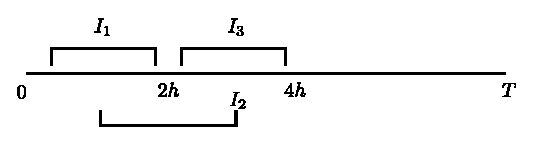
\includegraphics{figure/fig2.eps}
\end{figure}
$$
I_{k}=[(k-1)h,(k+1)h]\cap (0,T],\ k=1,2,\ldots .
$$

Let $I_{1},I_{2},\ldots I_{r}$ be those intervals for which
$$
I_{j}\cap [0,T]\neq \phi\,(j=1,2,\ldots,r).
$$

Clearly\pageoriginale there are $[\frac{T}{h}]+1$ of them. If
$|t-s|\leq h$ then $t$, $s\in I_{j}$ for some $j$, $1\leq j\leq
r$. Write $D=\bigcup\limits^{\infty}_{n=1}F_{n}$ where $F_{n}\subset
F_{n+1}$ and $F_{n}$ is finite. Then
\begin{align*}
& P_{x}\left\{\sup\limits_{\substack{|t-s|\leq h\\ t,s\in [0,T]\cap
      D}}|X(t)-X(s)|>\rho\right\}=P_{x}\left\{\bigcup^{\infty}_{n=1}\left(\sup\limits_{\substack{|t-s|\leq
  h\\ t,s\in D\cap F_{n}}}|X(t)-X(s)|>\rho\right)\right\}\\
&\qq =\sup\limits_{n}P_{x}\left\{\sup\limits_{j}\sup\limits_{t,s\in
    F_{n}}(|X_{I_{j}}(t)-X(s)|>\rho)\right\}\\
&\qq \leq \sup\limits_{n}\sum^{r}_{j=1}P_{x}\left(\sup\limits_{t,s\in
    F_{n}}(|X_{I_{j}}(t)-X(s)|>\rho)\right)\\
&\qq
  \sup\limits_{n}\left(\left[\frac{T}{h}\right]+1\right)\frac{C(2h)^{2}}{(\rho/4)^{4}}\q
  \text{by the last lemma}\\
&\qq \leq \phi(T,\rho,h).
\end{align*}
\end{proof}

\begin{theorem*}
$P_{x}(\Omega(D))=1$.
\end{theorem*}

\begin{proof}
It is enough to show that
$$
\Lt\limits_{j\to \infty}P_{x}\left(\Delta^{N,\frac{1}{j}}_{D}(f)\leq
\frac{1}{k}\right)=1\quad\text{(See Exercise \ref{chap4-exer4}(b)).}
$$

But this is guaranteed by the previous lemma.
\end{proof}

\begin{remark*}
\begin{enumerate}
\item It can be shown that the outer measure of $\Omega$ is $1$.

\item $\Omega$ is not measurable in $\prod\limits_{t\geq
  0}\mathbb{R}^{d}_{t}$. 
\end{enumerate}
\end{remark*}


Let\pageoriginale $\tilde{P}_{x}$ be the measure on $\Omega$ induced
by $P_{x}$ on $\Omega(D)$. We have already remarked that $P_{x}$ is
defined on the (topological Borel $\sigma$ field of $\Omega(D)$. As
$P_{x}$ is a probability measure, $\tilde{P}_{x}$ is also a
probability measure. It should now be verified that $\tilde{P}_{x}$ is
really the probability measure consistent with the given distribution.

\begin{theorem*}
$\tilde{P}_{x}$ is a required probability measure for a continuous
  realization of the Brownian motion.
\end{theorem*}

\begin{proof}
We have to show that
$$
F_{t_{1}\ldots t_{k}}=\tilde{P}_{x}\pi^{-1}_{t_{1}\ldots
  t_{k}}\quad\text{for all}\quad t_{1},t_{2}\ldots
t_{k}\quad\text{in}\quad [0,\infty).
$$


\setcounter{step}{0}
\begin{step}%1
Let $t_{1},\ldots,t_{k}\in D$. Then
$$
P_{x}(\pi^{-1}_{t_{1}\ldots t_{k}}(A_{1}\times\cdots\times
A_{k}))=P_{x}(\tau\pi_{t_{1}\ldots t_{k}}(A_{1}\times\cdots\times A_{k}))
$$
for every $A_{i}$ Borel in $\mathbb{R}^{d}$. The right side above is
$$
P_{x}(\pi^{-1}_{t_{1}\ldots t_{k}}(A_{1}\times\cdots\times
A_{k}))=F_{t_{1}\ldots t_{k}}(A_{1}\times\cdots\times A_{k})
$$
(by definition of $P_{x}$).
\end{step}

\begin{step}%2
We know that $T_{t_{1},t_{2}\ldots
  t_{k}}=\tilde{P}_{x}\pi_{t_{1},t_{2},\ldots,t_{k}}$ provided that
$t_{1},t_{2},\ldots,t_{k}\in D$. Let us pick
$t^{(n)}_{1},\ldots,t^{(n)}_{k}$, such that each $t^{(n)}_{i}\in D$
and $t^{(n)}_{k}\to t_{k}$ as $n\to \infty$. For each $n$ and for each
fixed $f:\mathbb{R}^{d}\to \mathbb{R}$ which is bounded and
continuous,
$$
E^{F^{(n)}_{1},\ldots t^{(n)}_{k}}[f(x_{1},\ldots,x_{k})]=E^{\tilde{P}_{x}}[f(x(t^{(n)}_{1},\ldots,x(t^{(n)}_{k})))].
$$
\end{step}

Letting\pageoriginale $n\to \infty$ we see that
$$
E^{F_{t_{1},\ldots,t_{k}}}[f(x_{1},\ldots,x_{k})]=E^{P_{x}}[f(x(t_{1}),\ldots,x(t_{k}))] 
$$
for all $t_{1},\ldots,t_{k}$. This completes the proof.
\end{proof}

The definition of the Brownian motion given earlier has a built-in
constraint that all ``trajectories'' start from $X(0)=x$. This result
is given by

\begin{theorem*}
$\tilde{P}_{0}\{f:f(0)=0\}=1$.
\end{theorem*}

\begin{proof}
Obvious; because $E^{\tilde{P}_{x}}[\phi(x(0))]=\phi(x)$.
\end{proof}

\begin{note*}
In future $\tilde{P}_{x}$ will be replaced by $P_{x}$ and
$\tilde{P}_{0}=P_{0}$ will be denoted by $P$.
\end{note*}

Let $T_{x}:\Omega\to \Omega$ be the map given by
$(T_{x}f)(t)=x+f(t)$. $T_{x}$ translates every `trajectory' through
the vector $x$.
\begin{figure}[H]
\centering
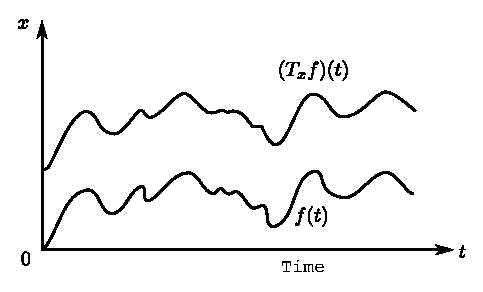
\includegraphics{figure/fig3.eps}
\end{figure}

Let us conceive a real Brownian motion of a system of particles. The
operation $T_{x}$ means that the system is translated in space (along
with everything else that affects it) through a vector $x$. The
symmetry of the physicl laws governing this motion tells us that any
property\pageoriginale exhibited by the first process should be
exhibited by the second process and vice versa. Mathematically this is
expressed by

\begin{theorem*}
$P_{x}=PT_{x}^{-1}$.
\end{theorem*}

\begin{proof}
It is enough to show that
$$
P_{x}(T_{x}\pi^{-1}_{t_{1}\ldots t_{k}}(A_{1}\times\cdots \times
A_{k}))=P(\pi^{-1}_{t_{1}\ldots t_{k}}(A_{1}\times\cdots\times A_{k}))
$$
for every $A_{i}$ Borel in $\mathbb{R}^{d}$. Clearly,
$$
T_{x}\pi^{-1}_{t_{1}\ldots t_{k}}(A_{1}\times\cdots\times
A_{k})=\pi^{-1}_{t_{1}\ldots t_{k}}(A_{1}-x\times\cdots \times
A_{k}-x).
$$

Thus we have only to show that
\begin{align*}
&\int_{A_{1}-x}\int\ldots \int_{A_{k}-x}p(0,x,t_{1},x_{1})\ldots
p(t_{k-1},x_{k-1},t_{k},x_{k})dx_{1}\ldots dx_{k}\\
&\q =\int_{A_{1}}\ldots \int_{A_{k}}p(0,0,t_{1},x_{1})\ldots
p(t_{k-1},x_{k-1},t_{k},x_{k})dx_{1}\ldots dx_{k},
\end{align*}
which is obvious.
\end{proof}

\begin{exer*}
\begin{enumerate}
\renewcommand{\theenumi}{\alph{enumi}}
\renewcommand{\labelenumi}{(\theenumi)}
\item If $\beta(t,\cdot)$ is a Brownian motion $s$ tarting at $(0,0)$
  then $\dfrac{1}{\sqrt{\epsilon}}\beta(\epsilon t)$ is a Brownian
  motion starting at $(0,0)$ for every $\epsilon>0$.

\item If $X$ is a $d$-dimensional Brownian motion and $Y$ is a
  $d'$-dimensio\-nal Brownian motion then $(X,Y)$ is a $d+d'$
  dimensional Brownian motion provided that $X$ and $Y$ are
  independent.

\item If $X_{t}=(X^{1}_{t},\ldots,X^{d}_{t})$ is a $d$-dimensional
  Brownian motion, then $X^{j}_{t}$ is a one-dimensional Brownian
  motion.\quad $(j=1,2,\ldots d)$.
\begin{align*}
\tau(w) &= \inf\{t:|X_{t}(w)|\geq +1\}\\
&= \inf\{t:|w(t)|\geq 1\}
\end{align*}\pageoriginale
$\tau(w)$ is the first time the particle hits either of the horizontal
lines $+1$ or $-1$.
\begin{figure}[H]
\centering
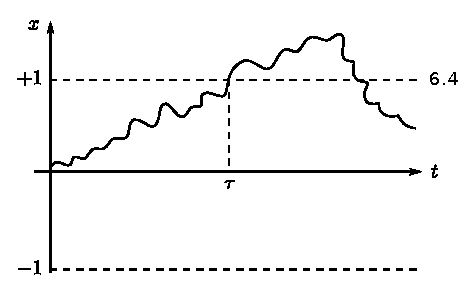
\includegraphics{figure/fig4.eps}
\end{figure}
\end{enumerate}

\begin{enumerate}
\setcounter{enumi}{1}
\item Let $\{X_{t}\}$ be a $d$-dimensional Brownian motion, $G$ any
  closed set in $\mathbb{R}^{d}$. Define
$$
\tau(w)=\inf\{t:w(t)\in G\}.
$$
This is a generalization of Example 1. To see that $\tau$ is a
stopping time use
$$
\{\tau\leq
s\}=\bigcap^{\infty}_{n=1}{\displaystyle{\mathop{\varlimsup}_{\substack{\theta\in
[0,s]\\ \theta\text{~ rational}}}}}\{w:w(\theta)\in G_{n}\},
$$
where
$$
G_{n}=\left\{x\in \mathbb{R}^{d}:d(x,G)\leq \frac{1}{n}\right\}.
$$

\item Let $(X_{t})$ be a $d$-dimensional Brownian motion, $C$ and $D$
  disjoint closed sets in $\mathbb{R}^{d}$. Define
$$
\tau(w)=\inf\{t;w(t)\in C\text{~ and for some~ }s\leq t,w(s)\in D\}.
$$
$\tau(w)$ is the first time that $w$ hits $C$ after visiting $D$.
\end{enumerate}
\end{exer*}


